\documentclass{article}
%
% PREFACE WITH INCLUDES, SETTINGS
% JUMP TO '\begin{document}' FOR ACTUAL CONTENT
%

\usepackage[utf8]{inputenc} % UTF8 encoding might save some debugging time
\usepackage{multicol} % for multiple columns
\setlength{\columnsep}{0.4cm} % sets the padding between colmuns
\usepackage{amssymb} % math symbols
\usepackage[table,dvipsnames]{xcolor} % colours

% hyperlinks
\usepackage{hyperref} 
\definecolor{linkcolor}{HTML}{0000EE}
\hypersetup{
  colorlinks=true,
  urlcolor=linkcolor,
  linkbordercolor=linkcolor,
  linkcolor=black,
  citecolor=black
}

% code snippets
\usepackage{listings} 
\lstdefinestyle{codeblock} {
    breaklines=true,
	basicstyle=\small\tt,
	keywordstyle=\color{RubineRed},
	showspaces=false,
	showstringspaces=false,
	stringstyle=\color{linkcolor},
    commentstyle=\color{ForestGreen}
}

% trees
\usepackage{forest}
\usepackage{tikz-qtree}
\forestset{
    default preamble={
    bold/.style={font=\bf},
    for tree={grow'=0, rectangle, anchor=west, parent anchor=east, child anchor=west, l=2.5cm, s sep=2pt, inner ysep=4pt}}
}

% page layout
\usepackage{geometry}
\geometry{a4paper,left=1.5cm, right=1.5cm, top=1cm, bottom=1.5cm} % page margins
\pagestyle{plain} % page numbering
\parindent=0pt % indentation after line breaks

% compact lists
\usepackage{enumitem}
\setlist{nolistsep}
\setlength{\itemindent}{-.5cm}

% to-dos
\newcommand{\todo}[1]{
    \textcolor{red}{$\bigstar$TODO: #1}
}



%
% CONTENT STARTS HERE
%
\begin{document}
\pagestyle{empty}

% title
\begin{center}
    \Large\bfseries Code On My Mind - \LaTeX\ Cheat Sheet
\end{center}

For beginners I recommend using templates and pasting your content in. Experiment with various formatting styles, maybe create a table and see where it goes from there. For a basic cheat sheet see: \url{https://wch.github.io/latexsheet/}. This is actually more of a collection of useful stuff with no claim of being complete.

% new section
\subsection*{Structure}
Organising your document is important. These commands will be useful friends in doing so:
\begin{multicols}{2}

    \begin{lstlisting}[style=codeblock]
\part{Part Title}
\section{Section Title}
\subsection{Small Section Title}
\subsubsection{Even Smaller Section Title}

Some Text.

Some Text on a new line.
    \end{lstlisting}
    
    \columnbreak\vfill
    
    \part{Part Title}
    \section{Section Title}
    \subsection{Small Section Title}
    \subsubsection{Even Smaller Section Title}

    Some Text.

    Some Text on a new line.

\end{multicols}
I recommend using a blank line to achieve a line break to make your code easier to read. Some prefer the double-backslash-method \verb|\\|

All commands are available with a $*$, which stops the automatic numbering. For example \verb|\section{Title}| turns into \verb|\section*{Title}|. Using the \href{http://tug.ctan.org/tex-archive/macros/latex/contrib/titlesec/titlesec.pdf}{titlesec} package will enable customisation of these structure elements.


% new section
\subsection*{Lists and Tables}
\begin{multicols}{2}
    \begin{lstlisting}[style=codeblock]
\begin{itemize}
    \item Unordered
    \item List
\end{itemize}
    \end{lstlisting}
    \columnbreak
    \begin{itemize}
        \item Unordered
        \item List
    \end{itemize}
\end{multicols}

\begin{multicols}{2}
    \begin{lstlisting}[style=codeblock]
\begin{enumerate}
    \item Ordered
    \item List
\end{enumerate}
    \end{lstlisting}
    \columnbreak
    \begin{enumerate}
        \item Ordered
        \item List
    \end{enumerate}
\end{multicols}
   
\begin{multicols}{2}
    \begin{lstlisting}[style=codeblock]
\begin{tabular}{l | c | r}
    Table & with & text-alignment \\
    \hline
    left & center & right
\end{tabular}
    \end{lstlisting}
    \columnbreak
    \begin{tabular}{l | c | r}
        Table & with & text-alignment \\
        \hline
        left & center & right
    \end{tabular}
\end{multicols}

Lists are implemented using the \texttt{itemize} or \texttt{enumerate} environments. The parameter \verb|{lcr}| for the \texttt{tabular} environment determines the alignment of the columns. Pipe symbols create a vertical line between columns - \verb|\hline| creates a horizontal line between rows. In case tables are too complicated, one can always use a \href{https://www.tablesgenerator.com/}{table generator}. 


% new section
\subsection*{Figures}
Most images are inserted using a figure. A short caption describes the image. A label will make referencing the image effortless \verb|\ref{label_name}|.

\begin{figure}[ht]
    \begin{center}
        
\includegraphics[width=.1\textwidth]{codeonmymind.png}
    \end{center}
    \caption{This text describes the image}
    \label{label_name}
\end{figure}

\begin{lstlisting}[style=codeblock]
\begin{figure}[ht]
    \begin{center}
        
\includegraphics[width=.1\textwidth]{codeonmymind.png}
    \end{center}
    \caption{This text describes the image}
    \label{label_name}
\end{figure}
\end{lstlisting}

The optional parameter \verb|[ht]| determines the figures float property. For a complete guide see \href{https://en.wikibooks.org/wiki/LaTeX/Floats,_Figures_and_Captions#Figures}{this wiki}.


% new section
\subsection*{Formatting Code}
The \href{http://texdoc.net/texmf-dist/doc/latex/listings/listings.pdf}{listings} package is the one I found most helpful. First 

\begin{lstlisting}[style=codeblock]
\usepackage{listings} 
\lstdefinestyle{codeblock} {
    breaklines=true,
    basicstyle=\small\tt,
    keywordstyle=\color{RubineRed},
    showspaces=false,
    showstringspaces=false,
    stringstyle=\color{blue},
    commentstyle=\color{ForestGreen}
}
\end{lstlisting}

And for the actual code snippet:

% This is where this guide got a little meta:
% I cannot display the code about lstlisting in a lstlisting-environment :)
{\small\verb|\begin{lstlisting}[style=codeblock, language=Python]|\\
\verb|    ...|\\
\verb|\end{lstlisting}|}

For inline code I recommend \verb|\verb|\texttt{|...|}, since it also escapes any LaTeX special characters.


% new section
\subsection*{New Command: TO DO}
\href{https://en.wikibooks.org/wiki/LaTeX/Macros}{New commands} are always defined before the actual document begins. Define name, number of arguments and the actual macro.
\begin{lstlisting}[style=codeblock]
\newcommand{\todo}[1]{
    \textcolor{red}{$\bigstar$TODO: #1}
}
\end{lstlisting}

Usage:
\begin{multicols}{2}
    \verb|\todo{Include to-do command in cheat sheet}|
    \columnbreak
    \todo{Include to-do command in cheat sheet}
\end{multicols}



% new section
\subsection*{Graphs}
For tree graphs, the \href{http://mirrors.ibiblio.org/CTAN/graphics/pgf/contrib/forest/forest-doc.pdf}{forest} package provides a compact syntax.
\begin{multicols}{2}
    \begin{lstlisting}[style=codeblock]
\begin{forest}
    [root[child,fill=red!20][child,fill=green!20][child,fill=blue!20]]
\end{forest}
    \end{lstlisting}
    \columnbreak
    \begin{forest}
    [root[child,fill=red!20][child,fill=green!20][child,fill=blue!20]]
    \end{forest}
\end{multicols}

A graphical method of creating any sort of graph is the \href{http://madebyevan.com/fsm/}{fsm tool}:
\begin{center}
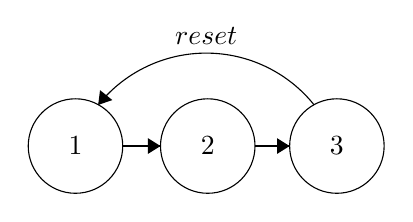
\begin{tikzpicture}[scale=0.2]
\tikzstyle{every node}+=[inner sep=0pt]
\draw [black] (33.5,-24.6) circle (3);
\draw (33.5,-24.6) node {$1$};
\draw [black] (41.9,-24.6) circle (3);
\draw (41.9,-24.6) node {$2$};
\draw [black] (50.1,-24.6) circle (3);
\draw (50.1,-24.6) node {$3$};
\draw [black] (36.5,-24.6) -- (38.9,-24.6);
\fill [black] (38.9,-24.6) -- (38.1,-24.1) -- (38.1,-25.1);
\draw [black] (44.9,-24.6) -- (47.1,-24.6);
\fill [black] (47.1,-24.6) -- (46.3,-24.1) -- (46.3,-25.1);
\draw [black] (34.945,-21.988) arc (141.27311:38.72689:8.787);
\fill [black] (34.94,-21.99) -- (35.84,-21.68) -- (35.06,-21.05);
\draw (41.8,-18.2) node [above] {$reset$};
\end{tikzpicture}
\end{center}


% new section
\subsection*{Detexify}
A really awesome tool. Draw any symbol to search for the corresponding latex command:

\url{http://detexify.kirelabs.org/classify.html}


% new section
\subsection*{German}
\verb|\usepackage{epsf,german}| will convert the language to german and will take care of any Umlaute issues.

\end{document}